\monster{Caos}{10}{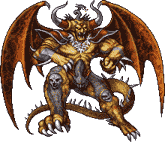
\includegraphics[width=0.23\textwidth]{./art/monsters/chaos.png}}
{
 PV: & \hfill 400 & PM: & \hfill 700 \\
 FUE: & \hfill 8 & DEF: & \hfill 8 \\
 MAG: & \hfill 10 & RES: & \hfill 7 \\
 AGI: & \hfill 4 & Tamaño: & \hfill G\\
}
{
 \textbf{Haz}: 5d de daño, 3u Alcance \hfill \textbf{Botín:} 10000 Gil \\
 \textbf{Inmune}: \hyperlink{status}{Todos los Estados Alterados} \\
 \textbf{Resistencia}:\dark\fire \mspell{Artema}{45}{3t}{3u}{5u}{
 Infliges 10d+10 de daño \hyperlink{type}{Oscuro} solo a los enemigos que se encuentren en el área de efecto. }{\dark} \mspell{Cura+++}{30}{2t}{3u}{5u}{
 Todos los aliados que se encuentren en el área de efecto recuperan 8d+10 de sus PV. }{} \mspell{Piro+++}{28}{2t}{3u}{8u}{
 Infliges 8d+10 de daño de \hyperlink{type}{Fuego} a todos los que se encuentren en el área de efecto. }{\fire}
 \mpassive{Toque Caótico}{
 Siempre que hagas un \hyperlink{action}{Ataque} con éxito, el objetivo debe hacer una tirada con DC 8. Si falla, sufre \hyperlink{status}{Veneno}, \hyperlink{status}{Ciego} y \hyperlink{status}{Silencio} por 3 turnos.
	}
 \mreaction{Acelerar}{
 Siempre que recibas daño, puedes hacer una tirada con DC 6. Si tienes éxito, tienes un turno adicional inmediatamente después del atacante. Este efecto no cambia el orden habitual de los turnos y solo puede utilizarse una vez por turno.
	}
	\vspace{0.1cm} \hrule \vspace{0.1cm} 
 "Pero renaceré una vez más. Así que aunque muera una y otra vez, yo regresaré. ¡Renacido en este ciclo infinito que he creado!" -- Caos }
